\documentclass[fontset=none]{ctexart}

\usepackage[T1]{fontenc}
\usepackage{fontspec}
\setCJKmainfont{SimSun}
% Latin Modern
\renewcommand*\ttdefault{txtt} % 改等宽字体

\setcounter{tocdepth}{5}
\setcounter{secnumdepth}{5}
% -1 part
% 0 chapter
% 1 section
% 2 subsection
% 3 subsubsection
% 4 paragraph
% 5 subparagraph

\usepackage{cite}
\usepackage{geometry}
\geometry{a4paper,scale=0.7}

\usepackage{algorithm}  
\usepackage{algorithmicx}  
\usepackage{algpseudocode}
\makeatletter
\newenvironment{breakablealgorithm}
  {% \begin{breakablealgorithm}
   \begin{center}
     \refstepcounter{algorithm}% New algorithm
     \hrule height.8pt depth0pt \kern2pt% \@fs@pre for \@fs@ruled
     \renewcommand{\caption}[2][\relax]{% Make a new \caption
       {\raggedright\textbf{\ALG@name~\thealgorithm} ##2\par}%
       \ifx\relax##1\relax % #1 is \relax
         \addcontentsline{loa}{algorithm}{\protect\numberline{\thealgorithm}##2}%
       \else % #1 is not \relax
         \addcontentsline{loa}{algorithm}{\protect\numberline{\thealgorithm}##1}%
       \fi
       \kern2pt\hrule\kern2pt
     }
  }{% \end{breakablealgorithm}
     \kern2pt\hrule\relax% \@fs@post for \@fs@ruled
   \end{center}
  }
\makeatother

\usepackage{amsmath}
\usepackage{amssymb}
\usepackage{graphicx}
\usepackage{subfigure}
\usepackage{changepage}
\usepackage{multirow}
\usepackage{url}

\usepackage{amsthm}
\newtheorem{theorem}{Theorem}[section]
\newtheorem{lemma}[theorem]{Lemma}
\newtheorem{proposition}[theorem]{Proposition}
\newtheorem{corollary}[theorem]{Corollary}
% \newtheorem{remark}{Remark}[section]
\newtheorem{example}{Example}[section]
\newenvironment{solution}{\begin{proof}[Solution]}{\end{proof}}
\theoremstyle{definition}
\newtheorem{definition}{Definition}[section]
\theoremstyle{remark}
\newtheorem*{remark}{Remark}

\usepackage[colorlinks, linkcolor=black, citecolor=blue, bookmarksnumbered]{hyperref}
% \hypersetup{
% 	colorlinks=true,
% 	linkcolor=cyan,
% 	filecolor=blue,      
% 	urlcolor=red,
% 	citecolor=green,
% }

\usepackage{fancyhdr}
\pagestyle{fancy}
\renewcommand{\sectionmark}[1]{\markright{\thesection\ #1}}
\fancyhf{}
\cfoot{\thepage}
\lhead{\rightmark}
% \rightmark 当前的节名
% \leftmark 当前的章名
% \(l/c/r)head{}, \(l/c/r)foot{}
\renewcommand{\headrulewidth}{0.4pt}
\renewcommand{\footrulewidth}{0pt}

\renewcommand\refname{References}
\renewcommand\contentsname{Content}
\renewcommand\figurename{Figure}

\begin{document}

\begin{titlepage}
    \begin{center}
        \vspace*{1cm}
            
        \Huge
        \textbf{Design and Implementation of A TTE System}
            
        \vspace{0.5cm}
        \LARGE
        Final Report\\
            
        \vspace{1.5cm}
            
        \textbf{11812804}  董\quad 正\\
        \textbf{11813225}  王宇辰\\
        \textbf{11811305}  崔俞崧\\

        \vspace{0.5cm}
        Supervisior: 宋轩
            
        \vfill
            
        
\includegraphics[width=\textwidth]{images/sustc.png}
            
        \vspace{0.2cm}
            
        \Large
        Department of Computer Science and Engineering\\
        \vspace{0.5cm}
        June 2021
            
    \end{center}
\end{titlepage}

\tableofcontents

\clearpage
\section{Preliminaries}
\subsection{Review}
\subsubsection{TTE}
\textbf{Travel Time Estimation (TTE)} is one of the most important researching topic in the traffic forecasting field. 
Estimating the travel time of any path in a city is of great importance to traffic monitoring, route planning, ridesharing, taxi dispatching, etc.
On Sep. 2020, DeepMind published a blog named \textit{Traffic prediction with advanced Graph Neural Networks}. 
This blog briefly described the whole industrial structure of estimated times of arrival (ETAs) techniques applied in Google Map but did not given any detailed implementation or any code.
Our work is based on the model structure of TTE proposed in the blog.
\begin{figure}[htb]
    \centering
    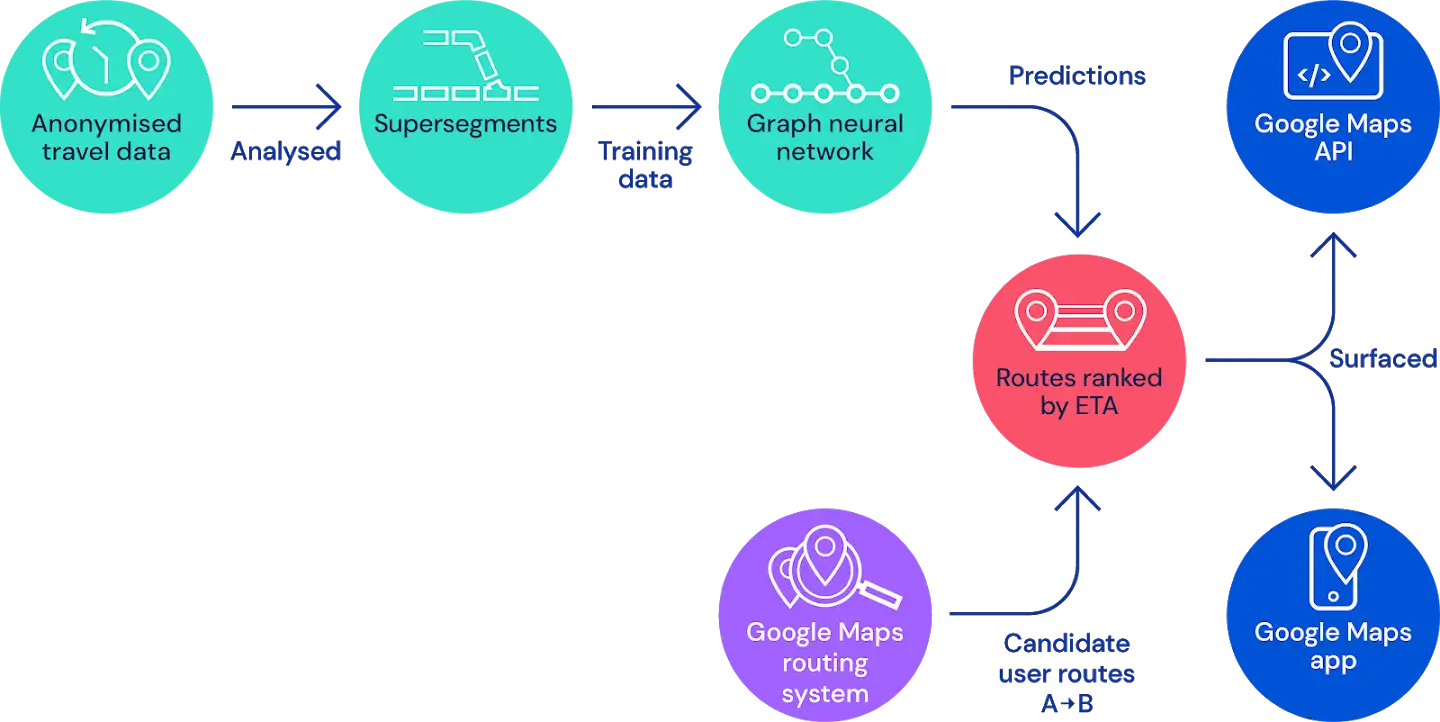
\includegraphics[width=0.9\textwidth]{images/architecture.png}
    \caption{Architecture}
    \label{fig1}
\end{figure}

\subsubsection{Goal}
Our ultimate goal (tentative) is to implement the industrial structure and apply it to the open source databases in China, then compare the performance with the state-of-the-art structures and find its application value.
This semester, we will implement a TTE system base on the work we done in the last term, combining \textit{Supersegment} and TTI.
We will try to work out an interactive application with graphical user interface. 

\subsection{Introduction}
In last stage, we completed the first version of our TTE web application.

Breifly, we will state our work in this report as
\begin{itemize}
  \item UI Redesign and Simple DB for TTE Web APP 董正 \& 王宇辰
  \item TTI Optimization by 崔俞崧
\end{itemize}

\section{UI Redesign and Simple DB for TTE Web APP}
\subsection{Introduction}
Our application is a front-back web system.
~\\

Front end:
\begin{itemize}
  \item \textit{Leaflet}: A JavaScript map library
  \item \textit{高德地图}: Provider of the base map
  \item \textit{jQuery}: A JavaScript communicator
\end{itemize}

Back end:
\begin{itemize}
  \item \textit{Flask}: A \textit{Python} back-end framework
  \item \textit{NetworkX}: A \textit{Python} library for graph analysis
  \item \textit{GeoJSON}: A special format of JSON that represents geo data
\end{itemize}

\subsection{System Overview}
\begin{enumerate}
  \item Convert orginal road data to \textit{shapefile} format
  \item Build geo-graph with \textit{NetworkX}
  \item Select start and end points in web front, use \textit{jQuery} to send request to back-end server
  \item Run \textit{Dijkstra} alogrithm in the graph to find shortest path and distance and store them in database
  \item Query database for the result
  \item Send \textit{GeoJSON} data to front-end and show the calculated path
  \item Calculate TTI, and use it to work out the estimated time of arrival
  \item Send the final result to front-end
\end{enumerate}

\begin{figure}[htb]
  \centering
  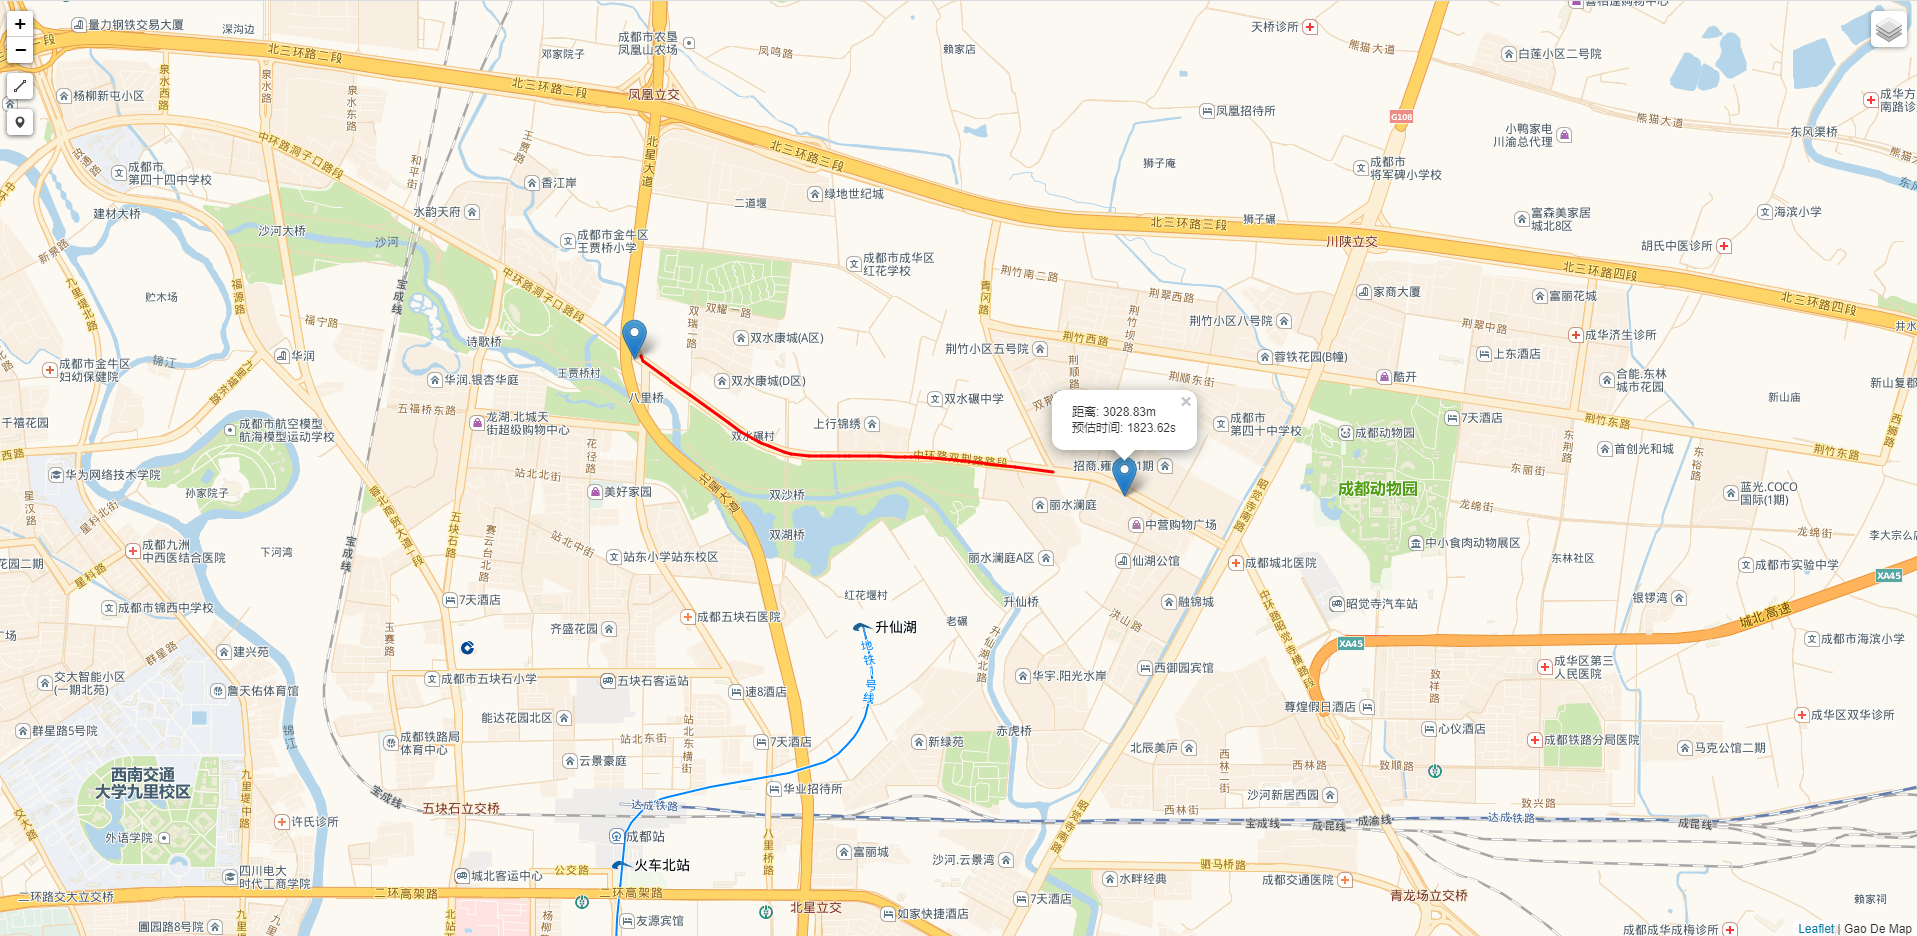
\includegraphics[width=\textwidth]{images/app_example_db.png}
  \caption{Web Application}
  \label{app}
\end{figure}

\subsection{Database Design}
For the ease of use, we designed a simple database with two tables.

\textbf{Table 1:}
\begin{itemize}
  \item Coordinate of the source point
  \item Coordinate of the target point
  \item Distance
  \item Path (a series of points)
\end{itemize}

\textbf{Table 2:}
\begin{itemize}
  \item Coordinate of the source point
  \item Coordinate of the target point
  \item Edge (contains road infomation)
\end{itemize}

\textbf{Database Interaction:}
\begin{enumerate}
  \item Input: Coordinates of the source point and target point
  \item Calculate the minimum of sum of manhattan distance to get the nearest points
  \item Query \textbf{Table 1} to get distance and path
  \item Use the path to query \textbf{Table 2} iteratively to get the roads
  \item Return distance and roads
\end{enumerate}

\begin{figure}[htb]
  \centering
  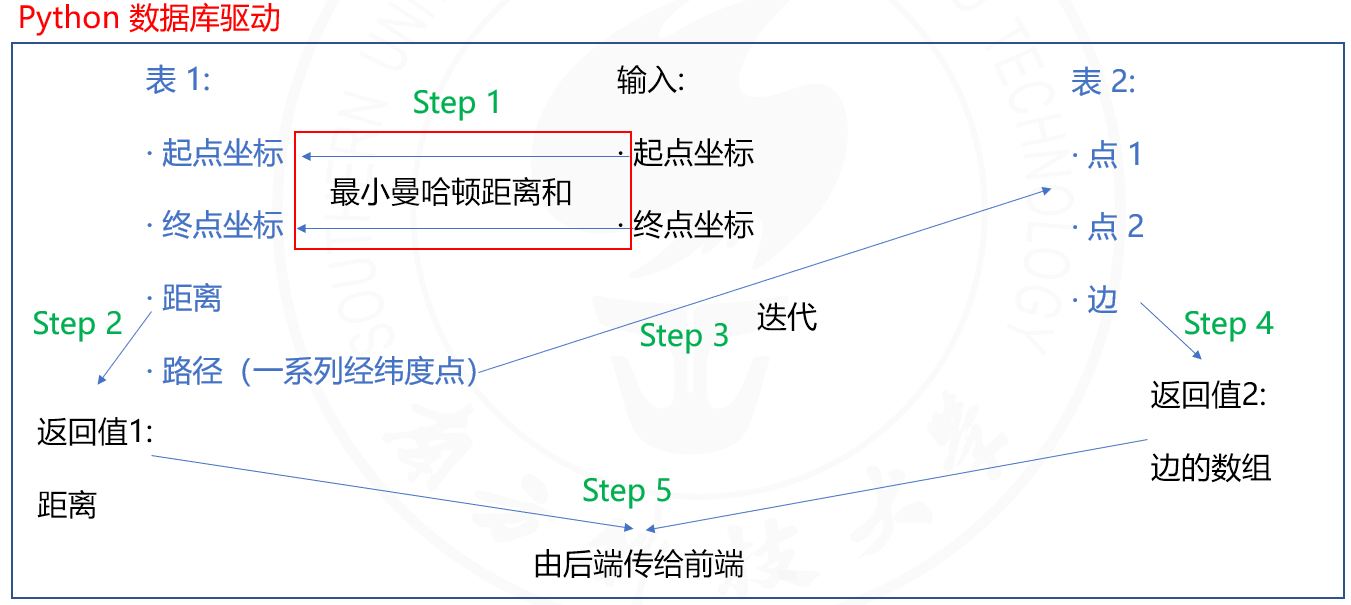
\includegraphics[width=\textwidth]{images/db_query.png}
  \caption{Database Query}
  \label{db}
\end{figure}

\section{TTI Optimization}
\subsection{Purpose Of TTI Optimization}
The main reason for TTI optimization is that several deficiencies of the current TTI calculation results are found in the actual application process, and the prediction accuracy could be improved by optimizing the current results.
First of all, when calculating unpopular road sections, it is easy to have no track records, which leads to null TTI value. 
Secondly, when the time granularity is finely divided, the adjacent values of TTI fluctuate greatly, and the results show a zigzag pattern, which will lead to large prediction errors.
Finally, the amount of data currently utilized is insufficient, resulting in the failure to utilize all the data effectively in the calculation. Data should be filtered reasonably to make full use of the data.

\subsection{TTI Optimization Methods}
\begin{enumerate}
  \item Complete TTI null values through interpolation. Due to the time limitation of adjacent TTI values, linear interpolation can be used when the null value is small. However, when the null value is large, the simple interpolation method cannot predict the TTI value of the void, and other ways are needed to complete it.
  \item Filtering is carried out after completion. Since the amount of data is not large, when the time granularity is fine, it is likely that the number of vehicles in each period is small, and the speed of different vehicles will vary greatly, so filtering is needed to reduce the impact caused by fluctuations and improve the accuracy.
  \item After interpolation, MAE, variance and other indicators are used to evaluate various filtering methods and select the best filtering method. MAE can be used to evaluate the distortion of TTI before and after filtering, while variance can be used to evaluate the effect of filtering.
\end{enumerate}

\clearpage
\subsection{TTI Optimization Process}
\begin{figure}[htb]
  \centering
  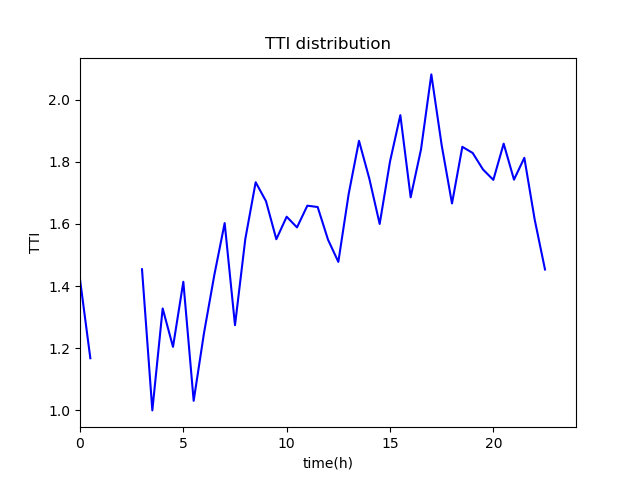
\includegraphics[width=0.8\textwidth]{images/6-3-1.png}
  \caption{TTI Without Processing}
  \label{6-3-1}
\end{figure}

\begin{figure}[htb]
  \centering
  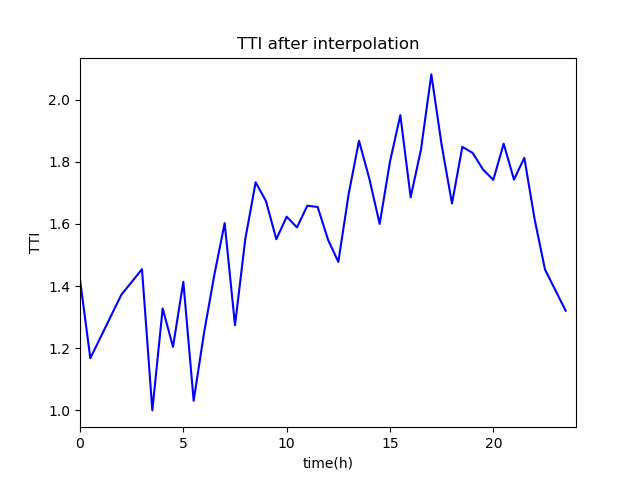
\includegraphics[width=0.8\textwidth]{images/6-3-2.png}
  \caption{TTI After Linear Interpolation}
  \label{6-3-2}
\end{figure}

\begin{figure}[htb]
  \centering
  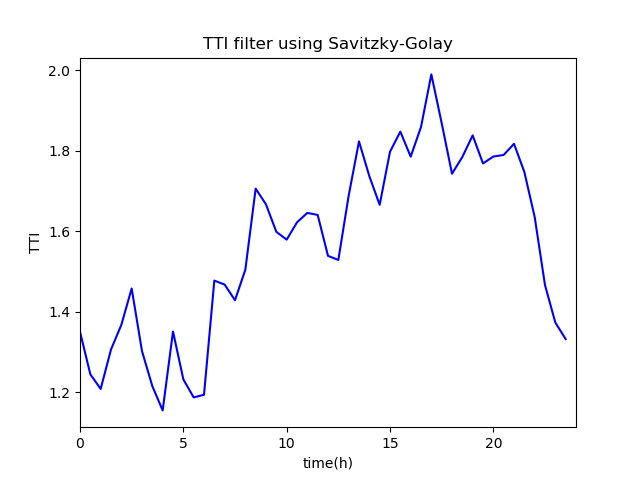
\includegraphics[width=0.8\textwidth]{images/6-3-3.png}
  \caption{TTI Filtering Using Savitzky-Golay}
  \label{6-3-3}
\end{figure}

\begin{figure}[htb]
  \centering
  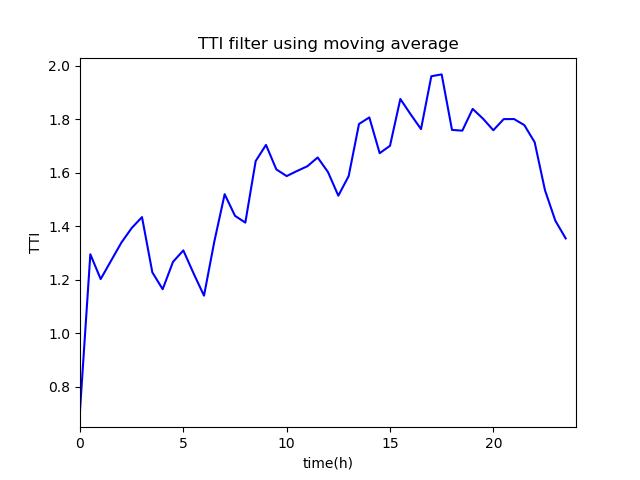
\includegraphics[width=0.8\textwidth]{images/6-3-4.png}
  \caption{TTI Filtering Using Moving Average}
  \label{6-3-4}
\end{figure}

\clearpage
\subsection{Result Analysis}
\begin{enumerate}
  \item It can be seen from the processing process of 3.3 that interpolation and filtering can fix the issue of null value and large fluctuation of TTI.
  \item The filtering results obtained by different filtering methods are different to some extent. A more appropriate filtering method can be obtained through comprehensive evaluation of various evaluation indexes.
  \item There are situations where the TTI result has many null values, and interpolation and filtering methods cannot be used at this time, and data processing should be considered.
  \item In order to ensure the efficiency of the algorithm, there is a certain error in the calculation process, and the processing of the results cannot eliminate the error in the calculation process.
\end{enumerate}

\subsection{Ascending Direction}
\begin{enumerate}
  \item Increase the amount of data and improve the efficiency of the algorithm, so that more data can be used to build the model and the algorithm can better deal with special cases.
  \item Since there are a large number of tracks from 8 am to 8 pm, and people are more likely to query the travel time during this period when using the app, this part of the time can be used instead of the using of whole time.
  \item When analyzing the TTI image, it is found that the TTI does not change much in the early morning of each day, and it is also the time when the null value and severe fluctuation are most likely to occur. Consider combining these periods to calculate the TTI.
\end{enumerate}

\clearpage
\section{Conclusion}
In this semester, we successfully builded a complete web application having front-end, back-end, and database. Still, its accuracy
needs to be improved. However, now it is ready for deployment and usage. Therefore, we achieved our goal proposed in the first report.

\begin{figure}[htb]
  \centering
  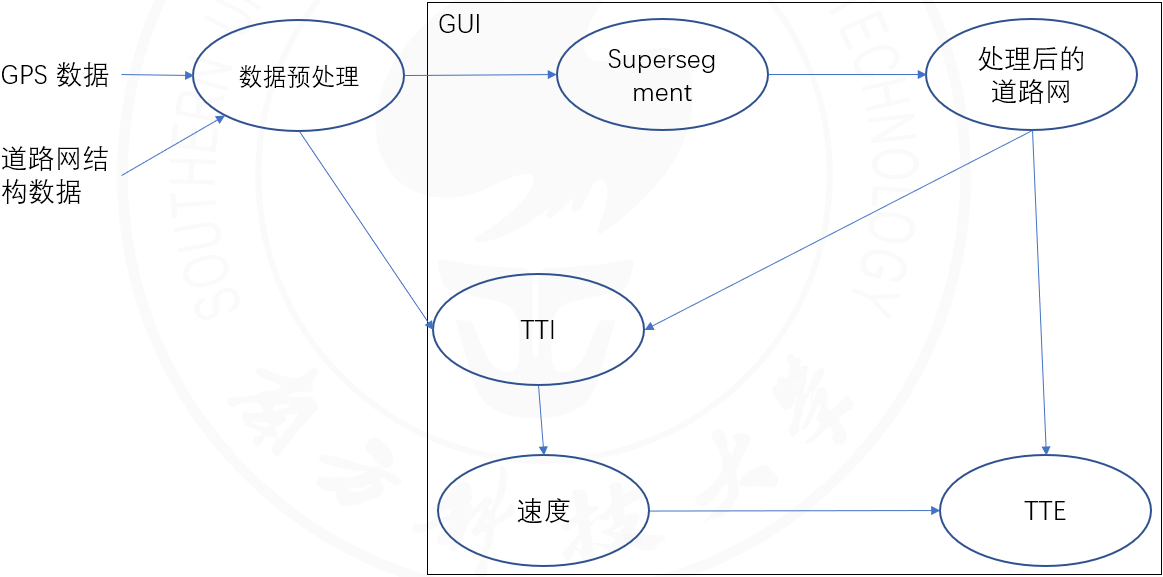
\includegraphics[width=\textwidth]{images/TTE_app_overview.png}
  \caption{TTE Web Application Structure}
  \label{web-application-structure}
\end{figure}

% \clearpage
% \phantomsection
% \addcontentsline{toc}{section}{References}
% \bibliographystyle{ieeetr}
% \bibliography{references}

\end{document}